\chapter{Validation of the Component Framework}
\label{chapter:applications}

In order to demonstrate the feasibility of the concepts of the framework and to meet Requirement
1 ``Simple User Interface'' (see Section \ref{chapter:requirements}), a test application which
utilizes and validates the Component Framework was implemented (cf. Section
\ref{sec:test_application}).

Furthermore, Mathias Breu� is using the Component Framework as basis for his bachelor thesis
\cite{scrumtool} to realize a complex component based (and therefore service oriented)
application (cf. Section \ref{sec:scrumtool}).

Finally, the Component Framework and the test application are analyzed in respect to the identified
requirements (cf. Section \ref{sec:solution_analysis}).

\section{Air Ambulance Test Application}
\label{sec:test_application}
To validate the developed Component Framework, a test application based on the air ambulance
scenario has been implemented. The test application can be seen as an interface to the Component
Framework using all its major functionalities (see Figure
\ref{fig:component_framework_user_interface}).

\begin{figure}
	\centering
		\fbox{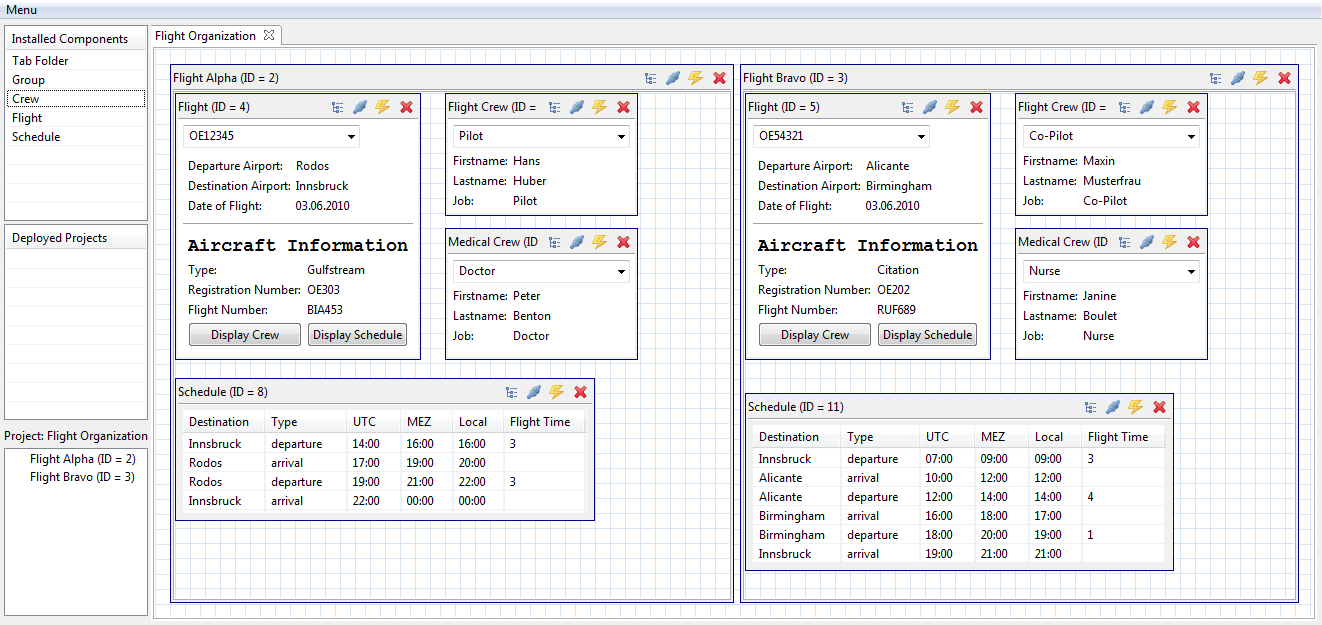
\includegraphics[width=1.2\textwidth,
		angle=90]{Bilder/test_application.png}}
	\caption{Test Application}
	\label{fig:component_framework_user_interface}
\end{figure}

The menu bar on top represents a direct link to the management agent functionality of the
component service and provides entries for installing component bundles and creating, saving, loading
and deploying projects.

On the left hand side the user interface provides information about installed component bundles,
deployed projects and the currently active components with respect to the selected project.
Additional context menus provide methods for uninstalling bundles and removing deployed projects.
Furthermore, the tables that display this information act as drag source. Therefore, other
components which implement a drop target can process the dragged data, as for example, the
``Group'' component does. It starts and displays the component and adds a menu bar for stopping the component again,
shifting it to another group component or connecting it with other components to directly exchange
data via the Component Wire Admin (see Section \ref{sec:wire_admin}).

The rest of the user interface is occupied by the working area, which is nothing else than a
tabfolder, where every tabitem constitutes a project. As soon as a new project is created and the
chosen project component is started, the user interface that is provided by the project component
(e.g., the group or tabfolder component) is placed on the tabitem. In the case of the displayed
example in Figure \ref{fig:component_framework_user_interface}, the project component is a
``Group'' component and the project is named ``Flight Organization''. Furthermore, the example
project has two child components, which are again ``Group'' components and hold the information of
two different flights. Therefore, the ``Flight Alpha'' and ``Flight Bravo'' components are populated
with different components which hold information about the flight, the airplane, the flight and
medical crew as well as about the detailed schedule. Both, the ``Crew'' and ``Schedule''
components receive their data from the ``Flight'' components by using the Wire and Event Admin
services (see Section \ref{sec:communication}).

\section{Scrumtool}
\label{sec:scrumtool}
For his bachelor thesis, Mathias Breu� developed a software product which is based on the described
test application and extends it with various custom components which should support Scrum teams
\cite{KS04} in the realization of software projects \cite{scrumtool}.

Figure \ref{fig:scrumtool} depicts the user interface of the test application which contains the
necessary custom components and extensively utilizes the provided complex components (see Section
\ref{sec:complex_components}) and hence the grouping and the launching of multiple
instances of a component functionality of the Component Framework. Furthermore, the scrumtool
transfers data from one component to the other by using the Wire Admin Service and requires the
Event Admin Service as well as the Event Information to propagate all kinds of events (see Section
\ref{sec:wire_admin}).

\begin{figure}
	\centering
		\fbox{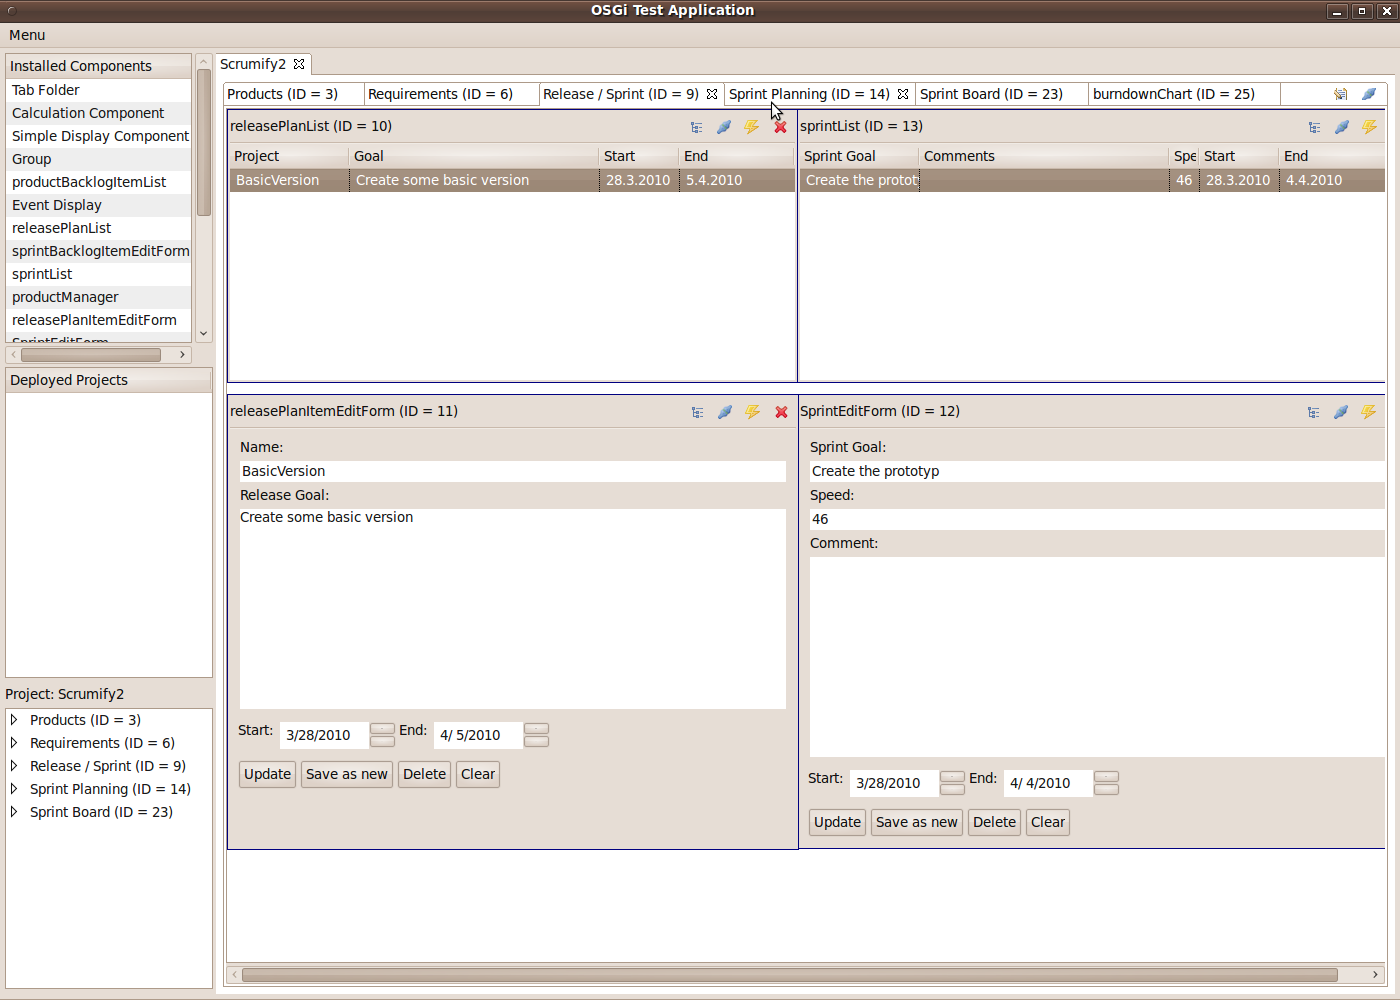
\includegraphics[width=0.98\textwidth]{Bilder/release_sprint.png}}
	\caption{Scrumtool}
	\label{fig:scrumtool}
\end{figure}

\section{Solution Analysis}
\label{sec:solution_analysis}
The ``Component Framework'' (see Section \ref{sec:component_framework}) was implemented to support
the identified requirements (see Section \ref{chapter:requirements}) and hence to provide a possible solution for
scenarios, like the air ambulance example which was introduced in Section \ref{sec:scenario}. The developed solution is
now analyzed to that effect.

\begin{itemize}
  \item \textbf{Simple User Interface}\newline The user interface which was developed for this master
  thesis is quite similar to the ones that are provided by the inspected mashup composers and adds
  the functionality to visually group components, to deploy these groups within other mashups or
  applications respectively and to install, start, stop and uninstall components. Summing up the
  user interface of the test application is easily operated and applies the popular drag and drop
  functions. Furthermore, it hides the complexity of the OSGi and Component Framework which
  encourages the user to create simple applications and mashups with a few mouse clicks.
  \item \textbf{Data Access and Processing}\newline As Java is the selected programming language and
  as the framework is highly extensible, components for most data sources can be easily implemented.
  That means that databases as well as Excel sheets, CSV files or even web services can be
  accessed.\newline However, the focus of this thesis was the implementation of a prototype framework
  and hence lacks many of these data access components. Anyhow, since the framework is easily
  extensible and provides a wizard for creating new components, additional data access components can
  be easily added.\newline In the context of data processing the Component Framework provides
  possibilities to directly connect two components via the Component Wire Admin (see Section
  \ref{sec:wire_admin}) or to publish events via the Event Admin and the Event Information Service
  (see Section \ref{sec:event_admin}) which are consumed by interested components. These mechanisms
  can be used to send and receive every kind of data and hence do not force the usage of a
  particular data format. However, it is possible to specify various preferred data formats, but if
  neither the data producer nor the consumer component can convert the data to one of these formats,
  an extra component has to be implemented, which performs the conversion.\newline That means that
  the Component Framework places the responsibility for eliminating data processing or compatibility
  problems on the end-user or component developer respectively.
  \item \textbf{Extensibility}\newline The Component Framework or the test application respectively
  provide a very limited number of pre-built blocks. Yet, these blocks offer powerful means for
  grouping components and reusing them within other applications in order to realize for example the
  monitoring of multiple airplanes in parallel (see Section \ref{sec:scenario}). Nevertheless, the
  framework has to be extended with custom blocks to make it applicable within specific usage
  scenarios.\newline To make the development of new components and hence the implementation of
  missing pre-built blocks and the extension of the Component Framework as easy as possible a wizard
  was implemented which generates the main classes and highlights the entry points for the custom
  code (see Section \ref{sec:component_implementation}). However, this requirement was already
  fulfilled by Microsoft Popfly and IBM Mashup Center and therefore does not constitute an advantage
  over existing mashup composer tools.
  \item \textbf{Running Multiple Instances of a Block}\newline As you can see in Section
  \ref{sec:test_application} the Component Framework allows the launching of multiple instances of
  components (e.g., the ``Flight'' or ``Crew'' components). This is realized by extending the OSGi
  Framework with the Component Starter and ID Service (see Section \ref{sec:component_starter_service}).
  \item \textbf{Grouping of Blocks}\newline The Component Framework provides great support for
  grouping of blocks via two different mechanisms (see Section \ref{sec:project}).\newline The first
  one is the concept of ``projects'', which can be compared to ``sites'' within IBM Mashup Center.
  For each project a tab is created which is filled with the chosen ``project component''. The test
  application therefore implements complex components (the ``Group'' and ``TabFolder'' components)
  which provide the possibility to drag and drop and arrange every kind of child component on
  them.\newline The second mechanism enables the grouping of components within projects. Therefore,
  the framework implements a parent child relationship and the components, which want to provide
  grouping functionality have to implement a form of display for the child components, like the
  described working area or a simple tabfolder, where each child constitutes a tabitem. That means
  that complex components can be used as ``project components'' and as child components of a
  ``project component'' and hence enable the nesting and grouping of components (cf. ``Flight Alpha''
  and ``Flight Bravo'' in Figure \ref{fig:component_framework_user_interface}).\newline Therefore,
  Requirement 5 ``Grouping of Blocks'' is fully supported and can be further enhanced by custom
  components.
  \item \textbf{Reusability of Groups}\newline Reusability of groups within the Component
  Framework is supported by enabling the deployment of projects within other projects or
  applications respectively. As soon as they are deployed, these projects are handled like simple
  groups within the new project and support the same life-cycle. Hence, they can be installed,
  started, stopped and uninstalled.
  \item \textbf{Hot Deployment and Life-cycle Management}\newline By using OSGi as underlying
  technological platform and extending it with the ``Component Service'', hot deployment and
  life-cycle management are enabled. Within the test application components are started by simply
  dropping them on a ``Group'' or ``TabFolder'' component and can be stopped at any time by using
  the provided menu bar, which is attached to every single component.
  \item \textbf{Event Management}\newline The event management service of the Component Framework
  encapsulates the basic functionality that is provided by the OSGi Framework and therefore enables
  the sending of events as well as the registration of components as Event Handlers for either
  single specific events or for groups of events. Furthermore, it extends the event mechanism by
  providing interfaces which should be implemented to expose human readable information about
  events (see Section \ref{sec:event_admin}). This alleviates the implementation of Event
  Handlers and makes the events processable correctly.
  \item \textbf{Logging}\newline The logging mechanism of the Component Framework enables the
  logging of errors, warnings and simple information, which can be analyzed by the component
  developers and reused to conduct data and process mining methods.
\end{itemize}
